\subsection{Nave}
\label{ship}

\begin{figure}[H]
	\centering
	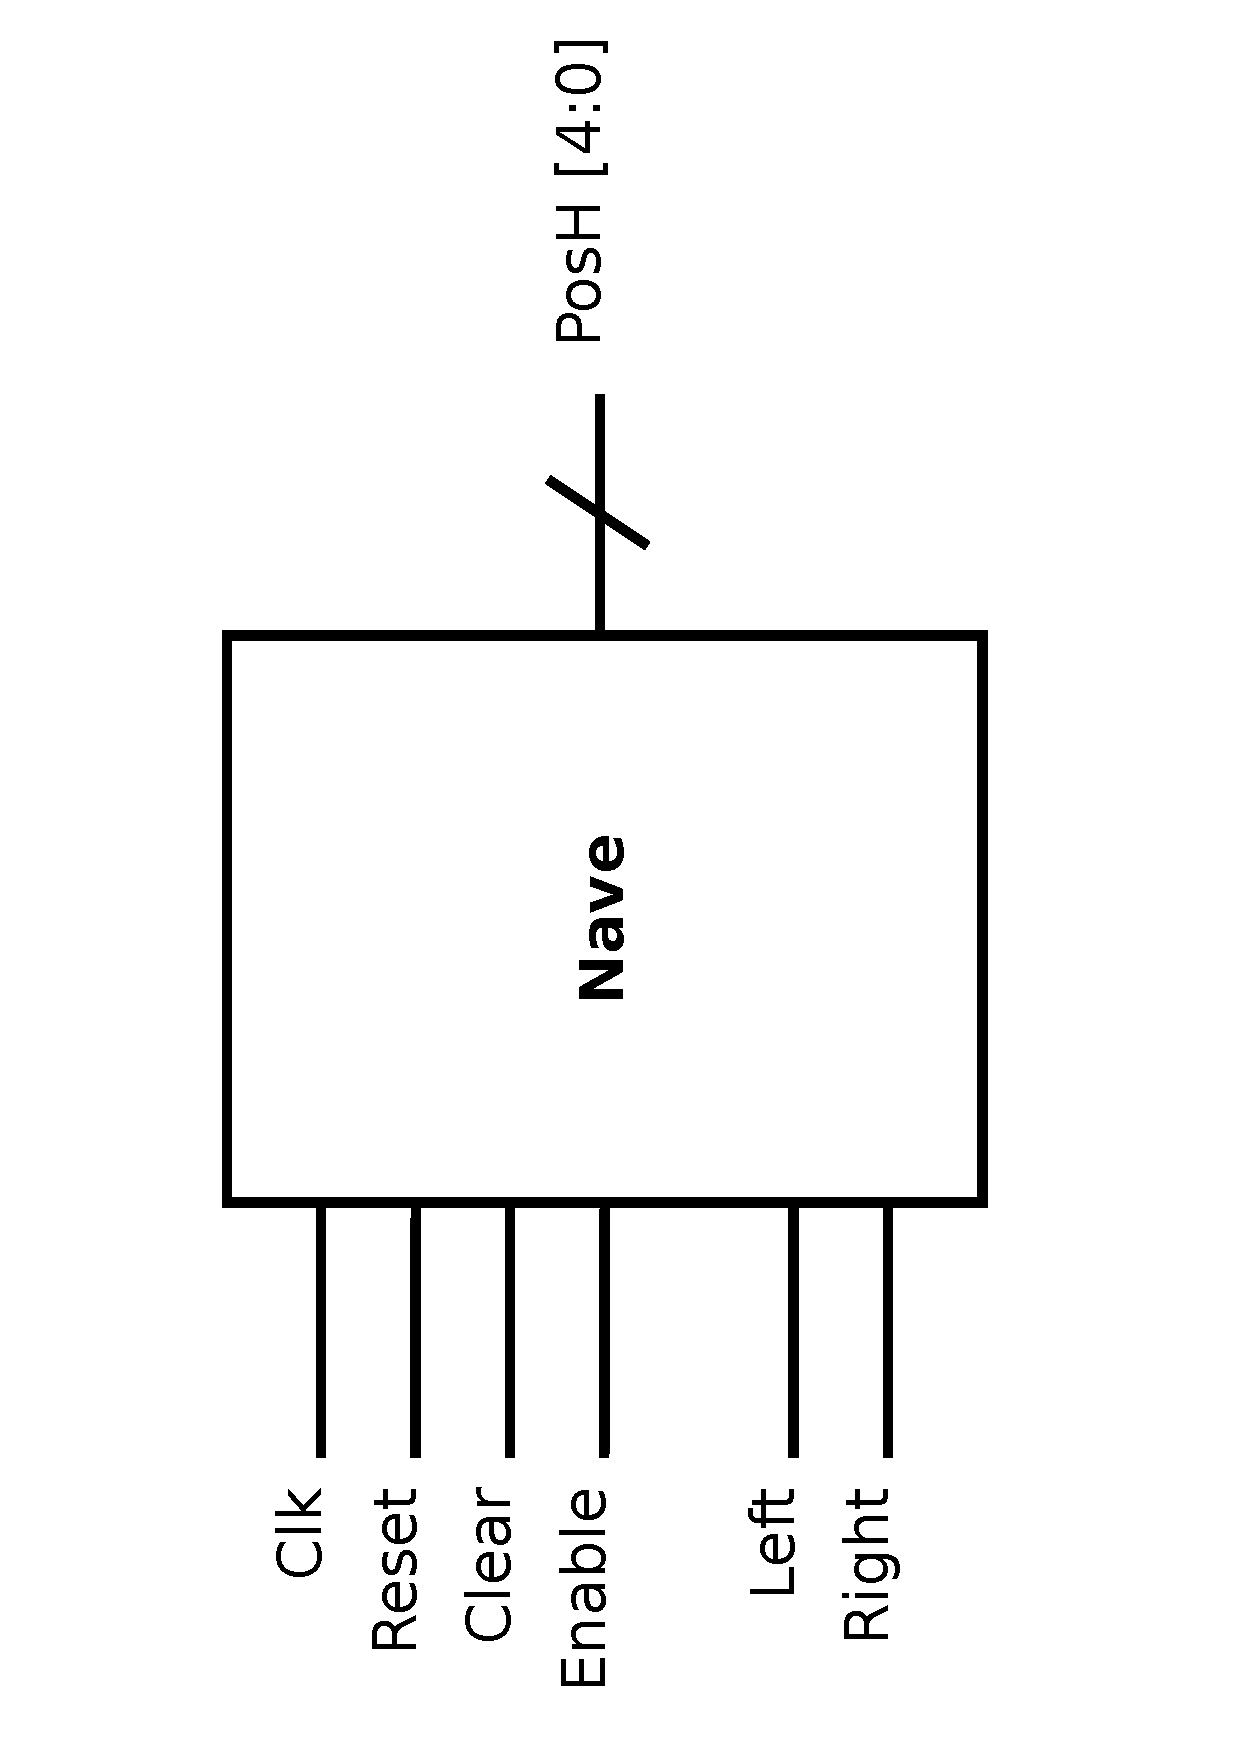
\includegraphics[width=0.4\textwidth, angle=-90] {ship_block.pdf}
	\caption{Interfaz de la entidad Nave}\label{fig:ship_block}
\end{figure}


La entidad \textit{nave} controla el movimiento de cada usuario sobre la pantalla de juego. Es parte de la entidad \textit{Jugador}.

El movimiento de la nave es controlado por las señales \textit{left} y \textit{right}, siempre y cuando no se haya alcanzado los límites de la pantalla. La señal \textit{enable} (conectada a un temporizador externo) limita la velocidad de movimiento de la nave.

La posición de la nave se codifica en la señal de 5 bits \textit{posH}, que se usa tanto para mostrarla en la pantalla como para indicar a la entidad \textit{Bala} la posición de disparo.

\subsubsection{Testbench}
El banco de pruebas \texttt{spaceship\_tb.vhd} comprueba el correcto funcionamiento de la nave en cualquier dirección y que no sobrepasa los límites de la pantalla.